% ********** Rozdział 4 **********
\chapter{Prezentacja warstwy użytkowej projektu}

\section{Logowanie}

Uruchamiając aplikację, użytkowniku wyświetla się okno logowania:

\begin{figure}[H]
\begin{center}
    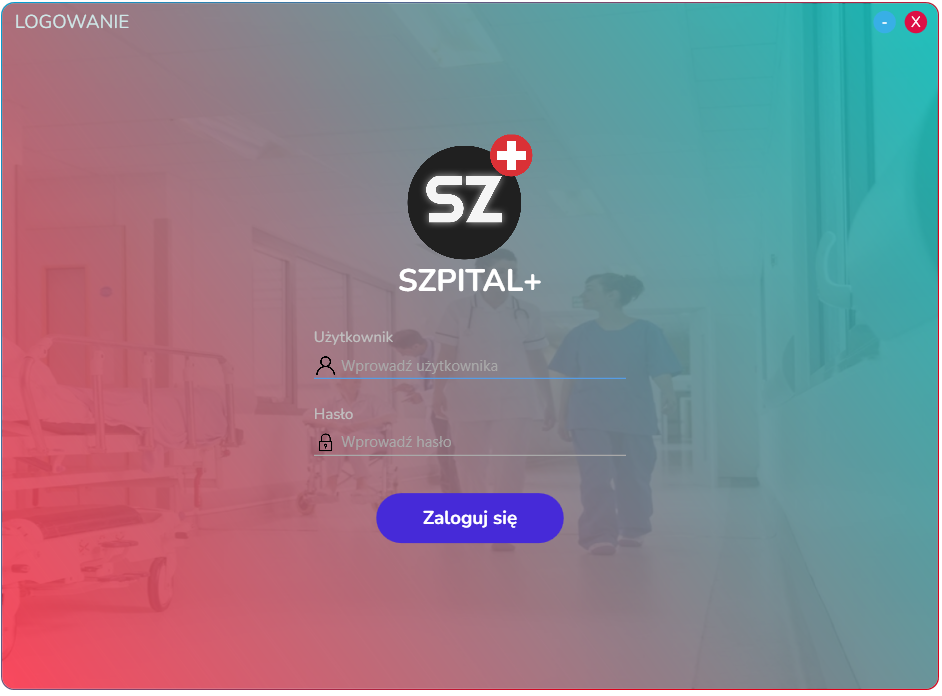
\includegraphics[height=10cm]{images/log_widok.png}
    \caption{Okno logowania}
\end{center}
\end{figure}

W tym oknie został przerobiony górny standardowy panel aplikacji windows. Rozmiar okna 750x550px. Także tło oraz granica zrobione z gradientu. Okno jest trochę zaokrąglone. Po wprowadzeniu danych i naciśnięciu przycisku \textquotedbl Zaloguj się\textquotedbl{} klasa statyczna DbContext sprawdza czy użytkownik istnieje i czy hasło jest poprawne za pomocą polecenia SQL. W przypadku gdy użytkownik poda błędne dane DbContext rzuca wyjątek \textquotedbl UserIdentifyException\textquotedbl{} który jest łapany w LoginCommand, skąd wypisuje się komunikat.

\begin{figure}[H]
\begin{center}
    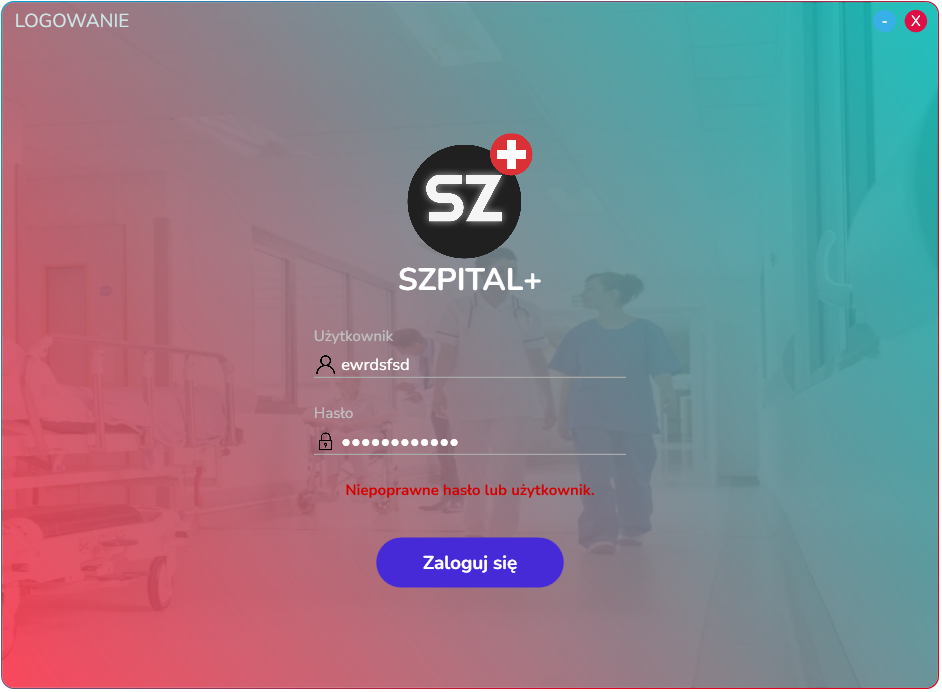
\includegraphics[height=10cm]{images/niep_uzyt.png}
    \caption{Wprowadzenie błędnych danych do logowania}
\end{center}
\end{figure}

Jeśli użytkownik istnieje i hasło jest poprawne —logujemy się do aplikacji.

\begin{figure}[H]
    \centering
    \subfigure{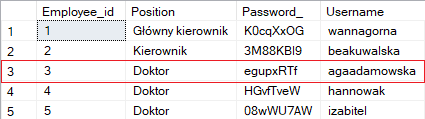
\includegraphics[width=0.6\textwidth]{images/istn_uzyt.png}} 
    \subfigure{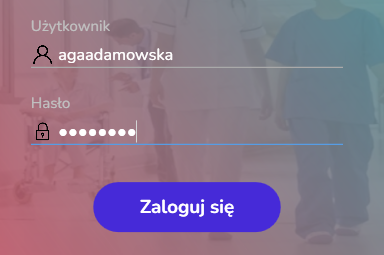
\includegraphics[width=0.3\textwidth]{images/rand_uzyt1.png}}
    \subfigure{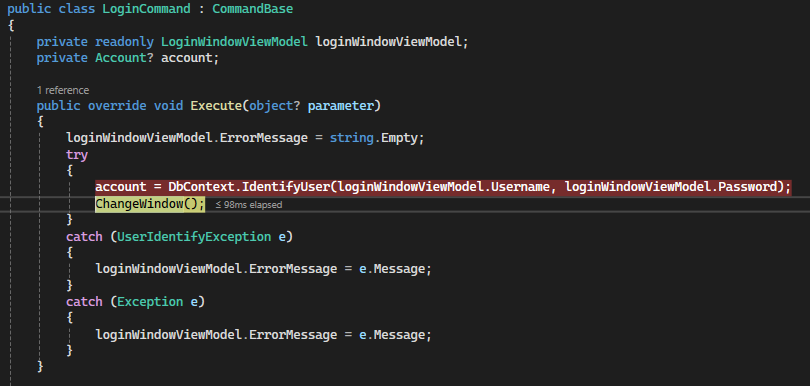
\includegraphics[width=0.8\textwidth]{images/log_kom_exe.png}}
    \caption{Logowanie (DbContext nie rzucił wyjątku)}
\end{figure}

\section{Główne okno}

MainWindow(Okno główne) składa się z trzech części:

\begin{figure}[H]
\begin{center}
    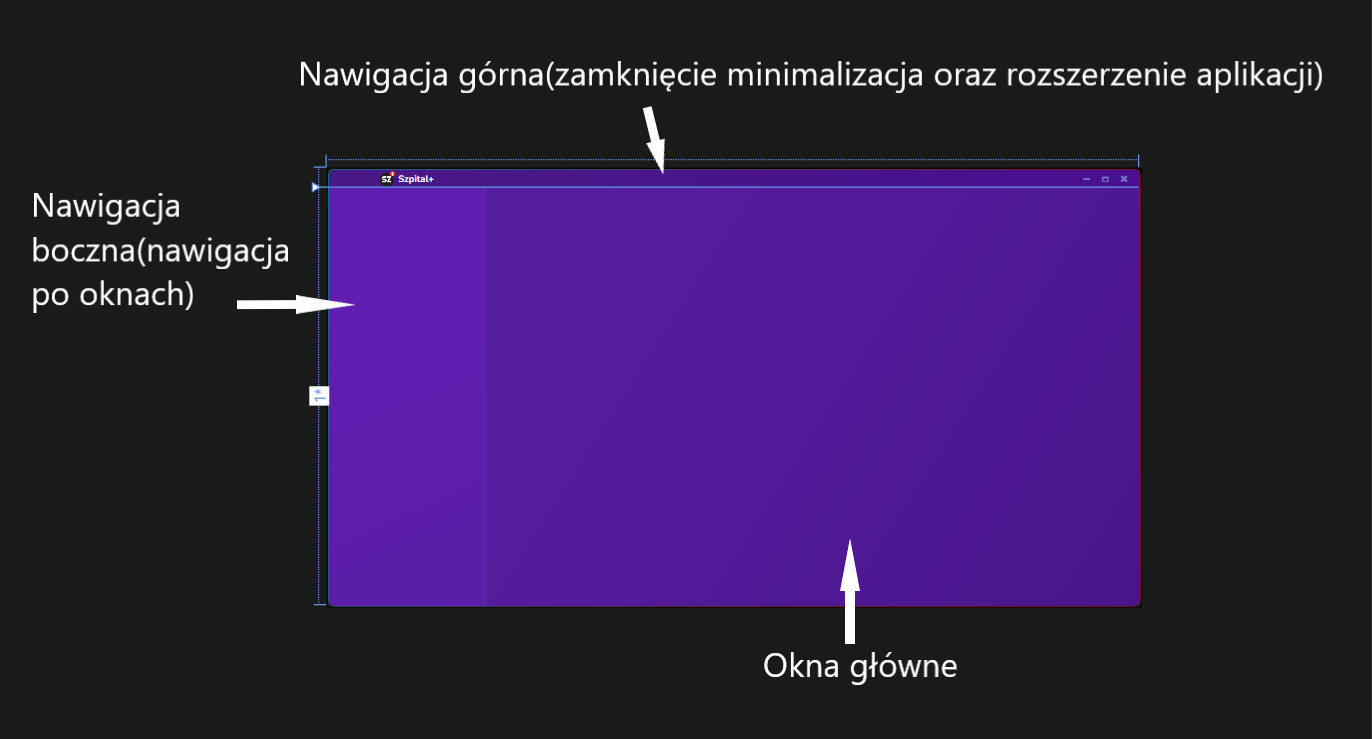
\includegraphics[height=8cm]{images/mainwindow.png}
    \caption{Główne okno}
\end{center}
\end{figure}

Aplikacja pobiera dane z bazy i ze względu na to, na jakim stanowisku pracuje użytkownik, wykorzystuje jeden z szablonów dotyczący jego posady żeby stworzyć nowy wygląd nawigacji bocznej.

\begin{figure}[H]
\begin{center}
    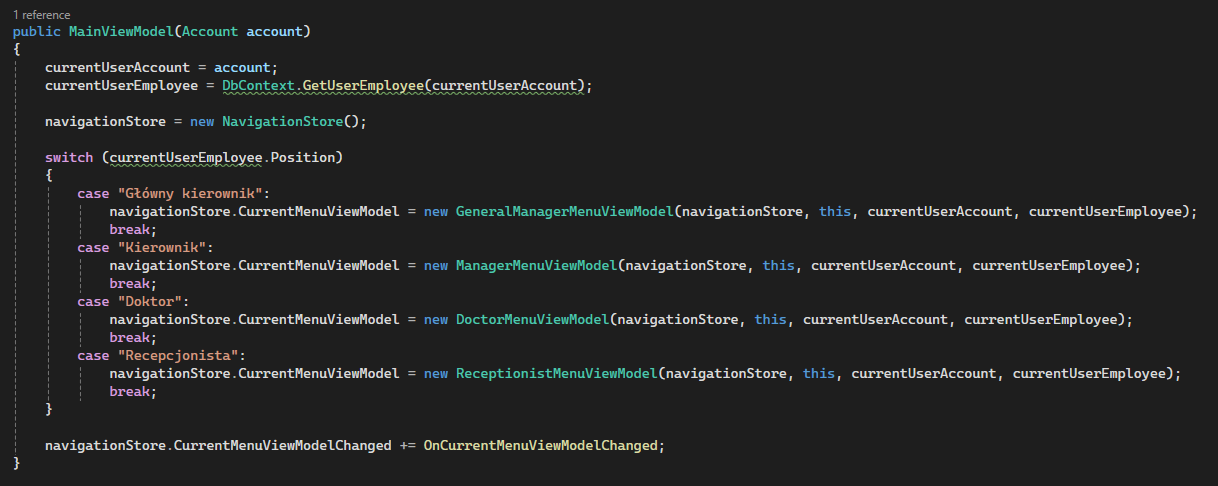
\includegraphics[height=7cm]{images/mainviewmodel_const.png}
    \caption{Pobieranie stanowiska użytkownika i przypisanie nowego wyglądu}
\end{center}
\end{figure}

Na przykład do aplikacji został zalogowany Recepcjonista.
Wtedy wygląd jego aplikacji będzie następny(także aplikacja sprawdza jaki zwrot wykorzystać na pulpicie ze względu na płeć osoby):

\begin{figure}[H]
\begin{center}
    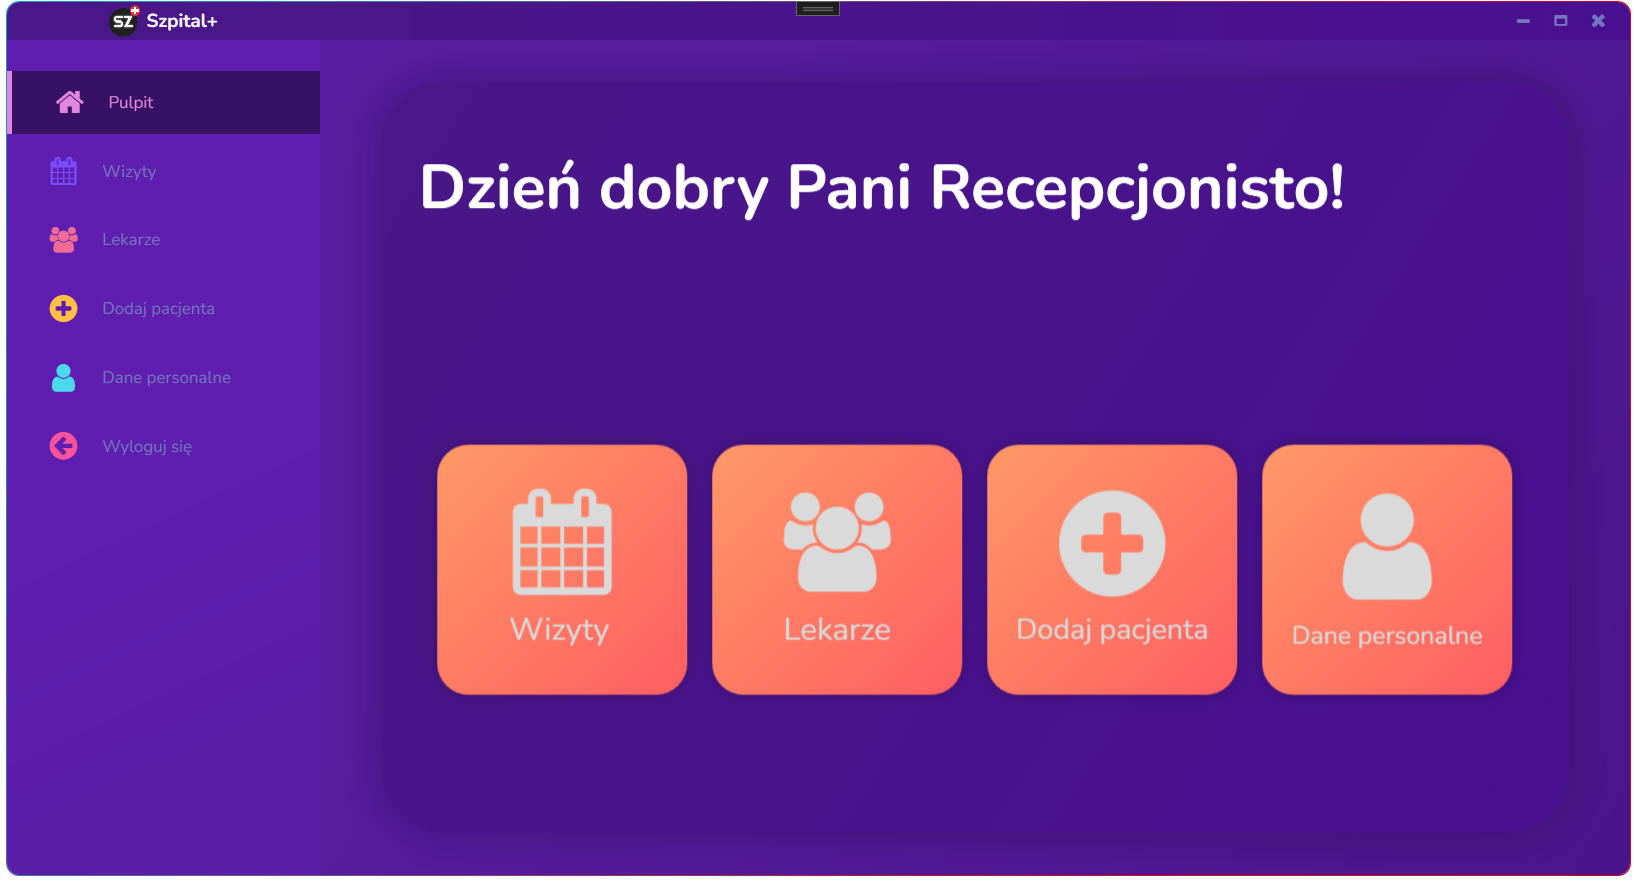
\includegraphics[height=8cm]{images/recep_view.png}
    \caption{Wygląd aplikacji recepcjonisty(Katarzyna Pabiniak)}
\end{center}
\end{figure}

\begin{figure}[H]
\begin{center}
    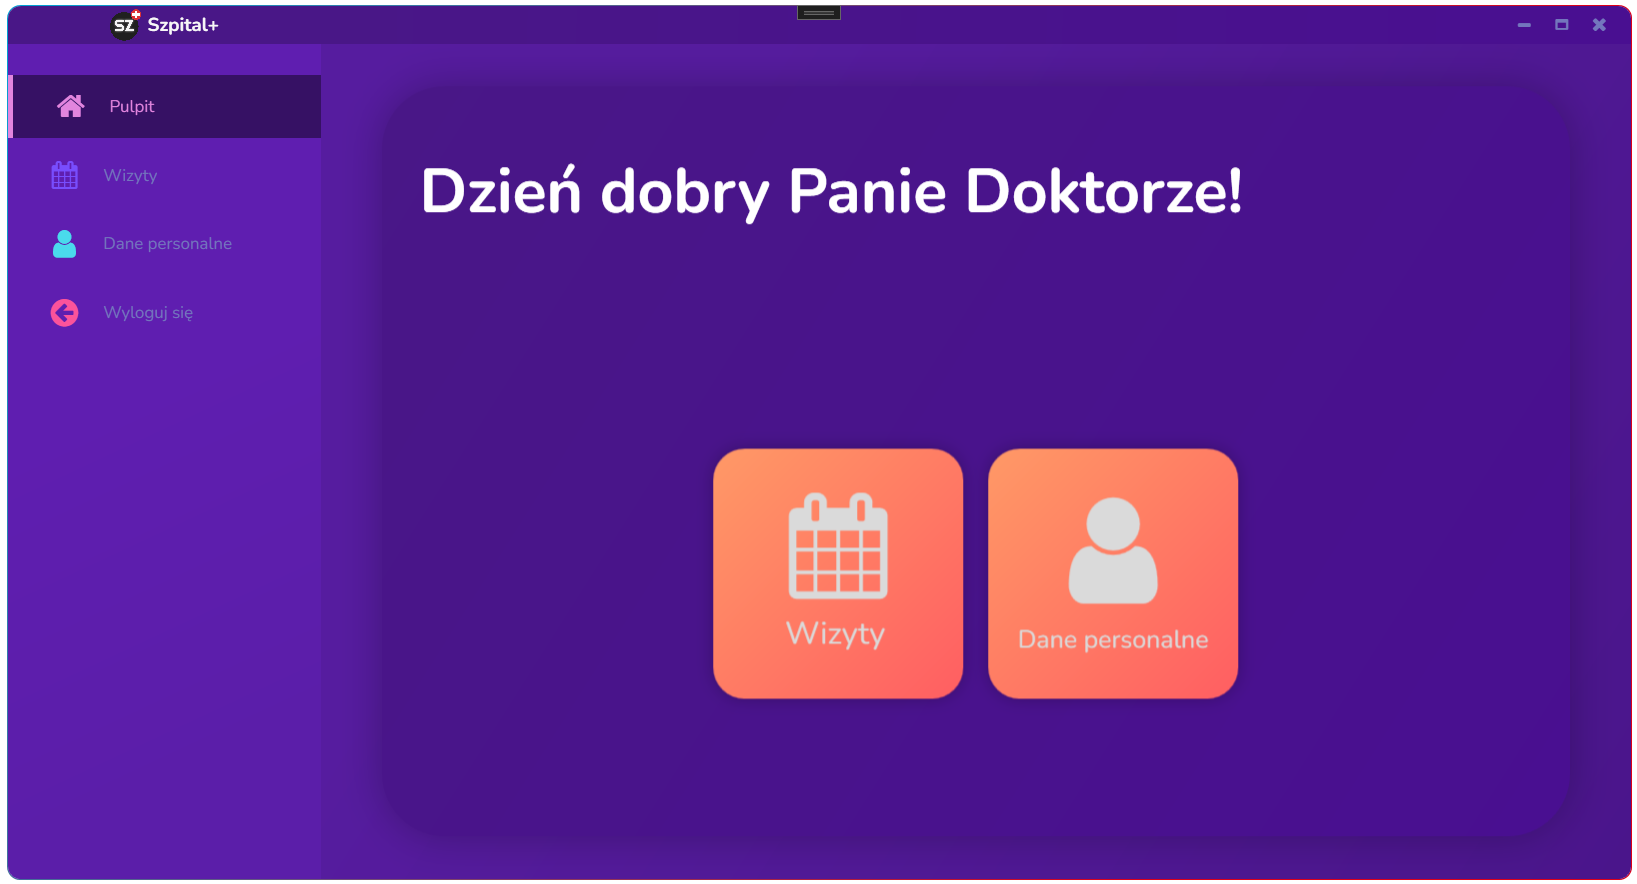
\includegraphics[height=8cm]{images/doktor_view.png}
    \caption{Wygląd aplikacji doktora(Filip Jabcoń)}
\end{center}
\end{figure}

Każdy klient na panelu nawigacyjnym bocznym ma przyciski: pulpit(okno z nawigacją), dane personalne(dane o użytkowniku), wyloguj się(wylogowanie z systemu i wracanie do okna logowania).

\section{Dane personalne}

\begin{figure}[H]
    \centering
    \subfigure{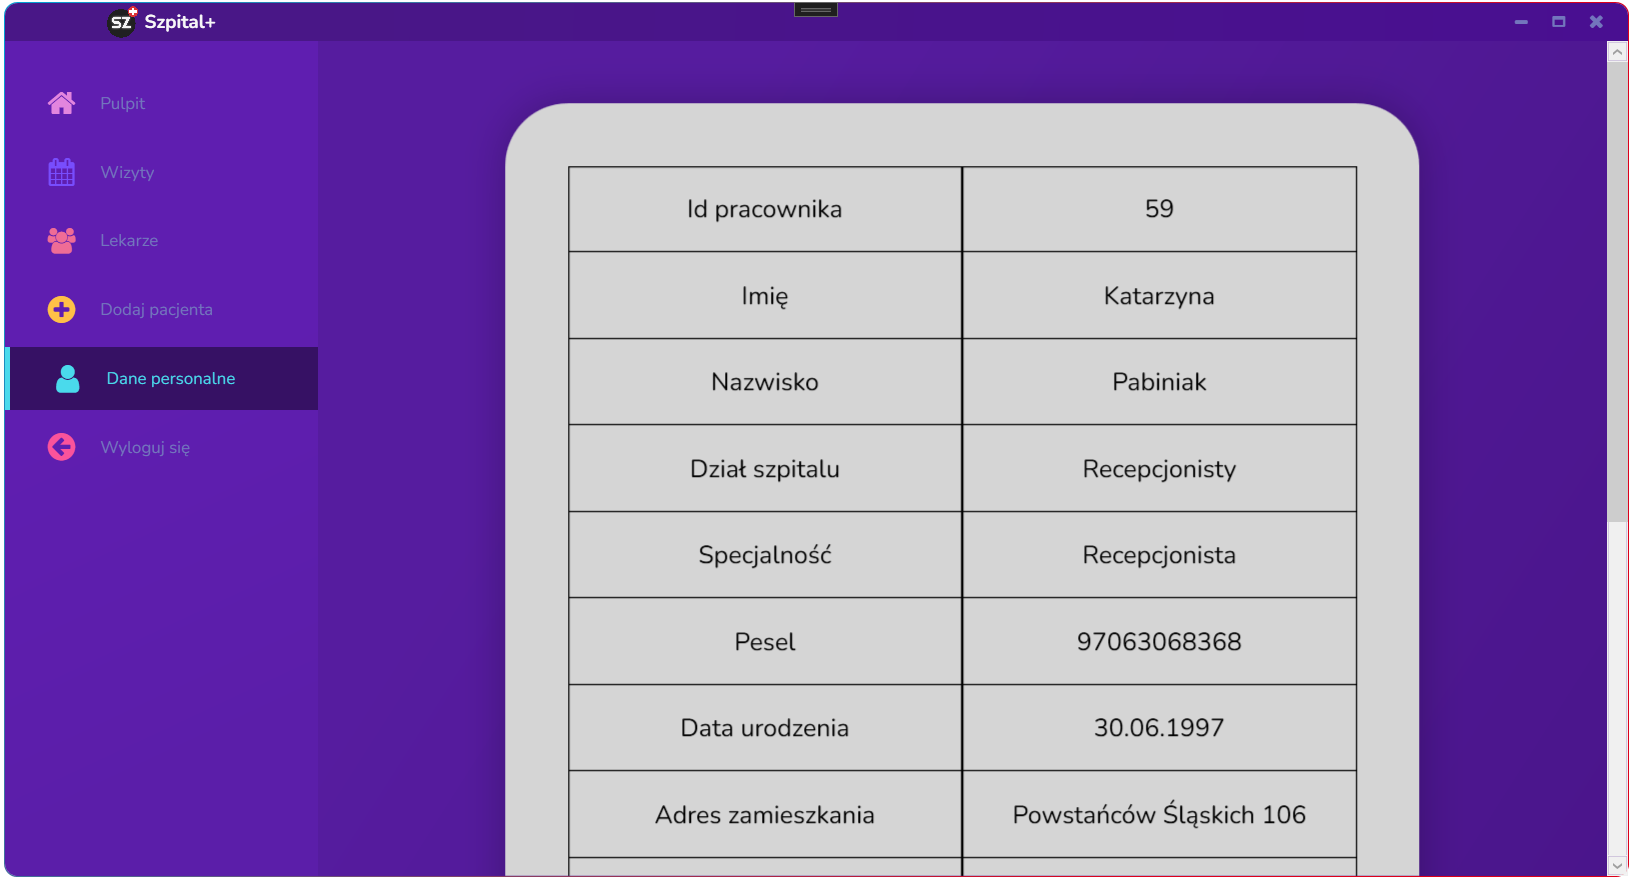
\includegraphics[width=0.7\textwidth]{images/dane_person1.png}} 
    \subfigure{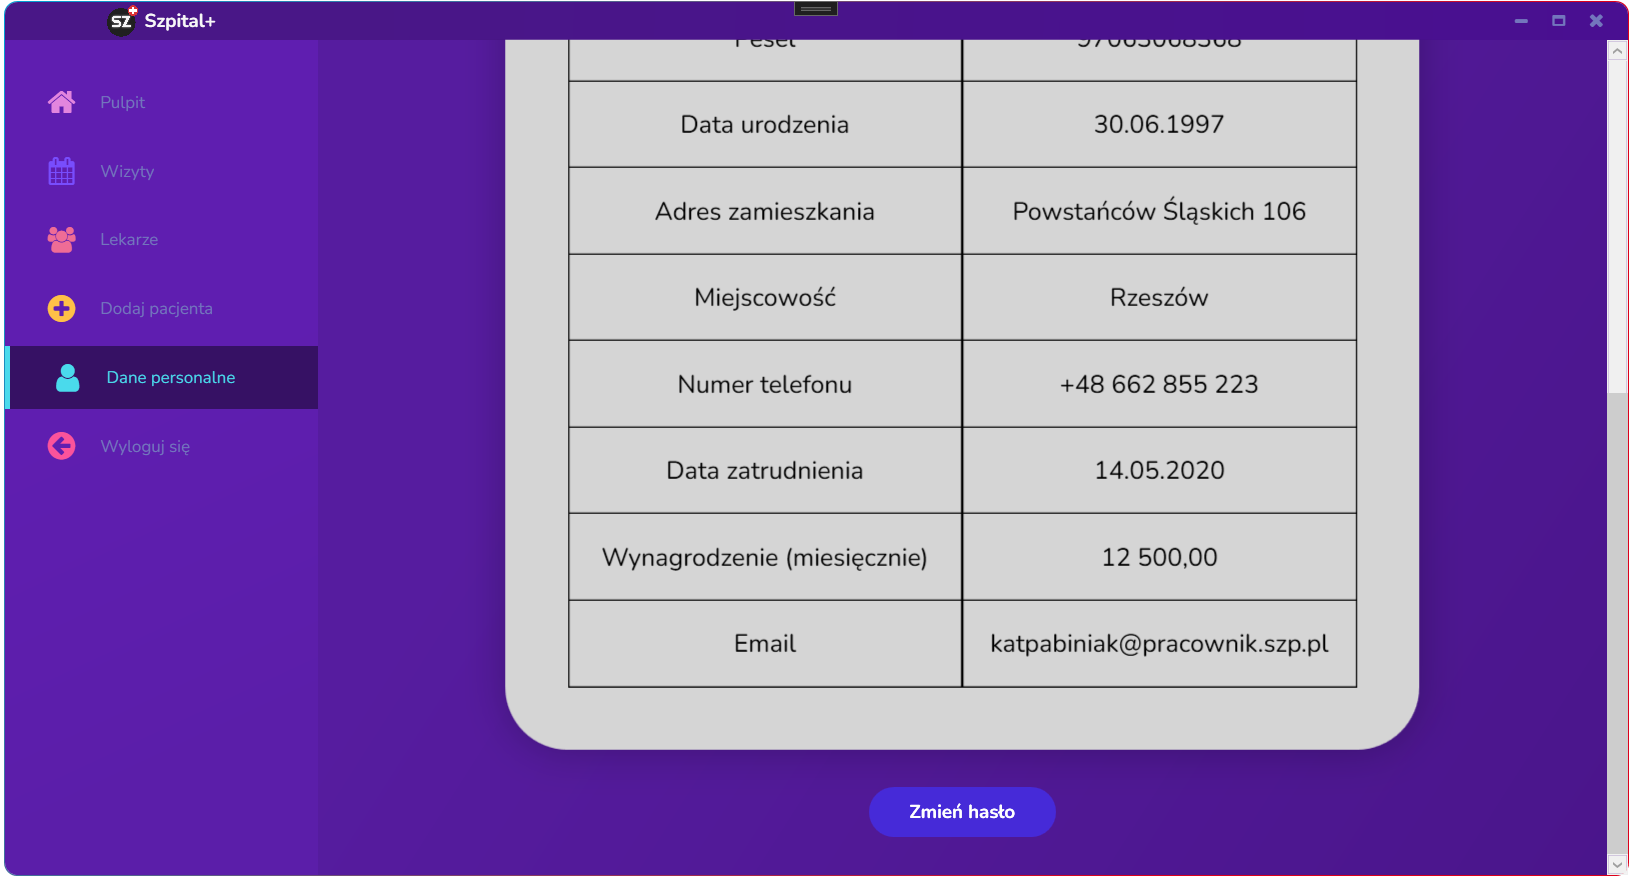
\includegraphics[width=0.7\textwidth]{images/dane_person2.png}}
\caption{Wygląd danych personalnych}
\end{figure}

\section{Zmienianie hasła}

Zmienianie hasła dostępne na dołu okna Dane personalne za pomocą przycisku.

\begin{figure}[H]
\begin{center}
    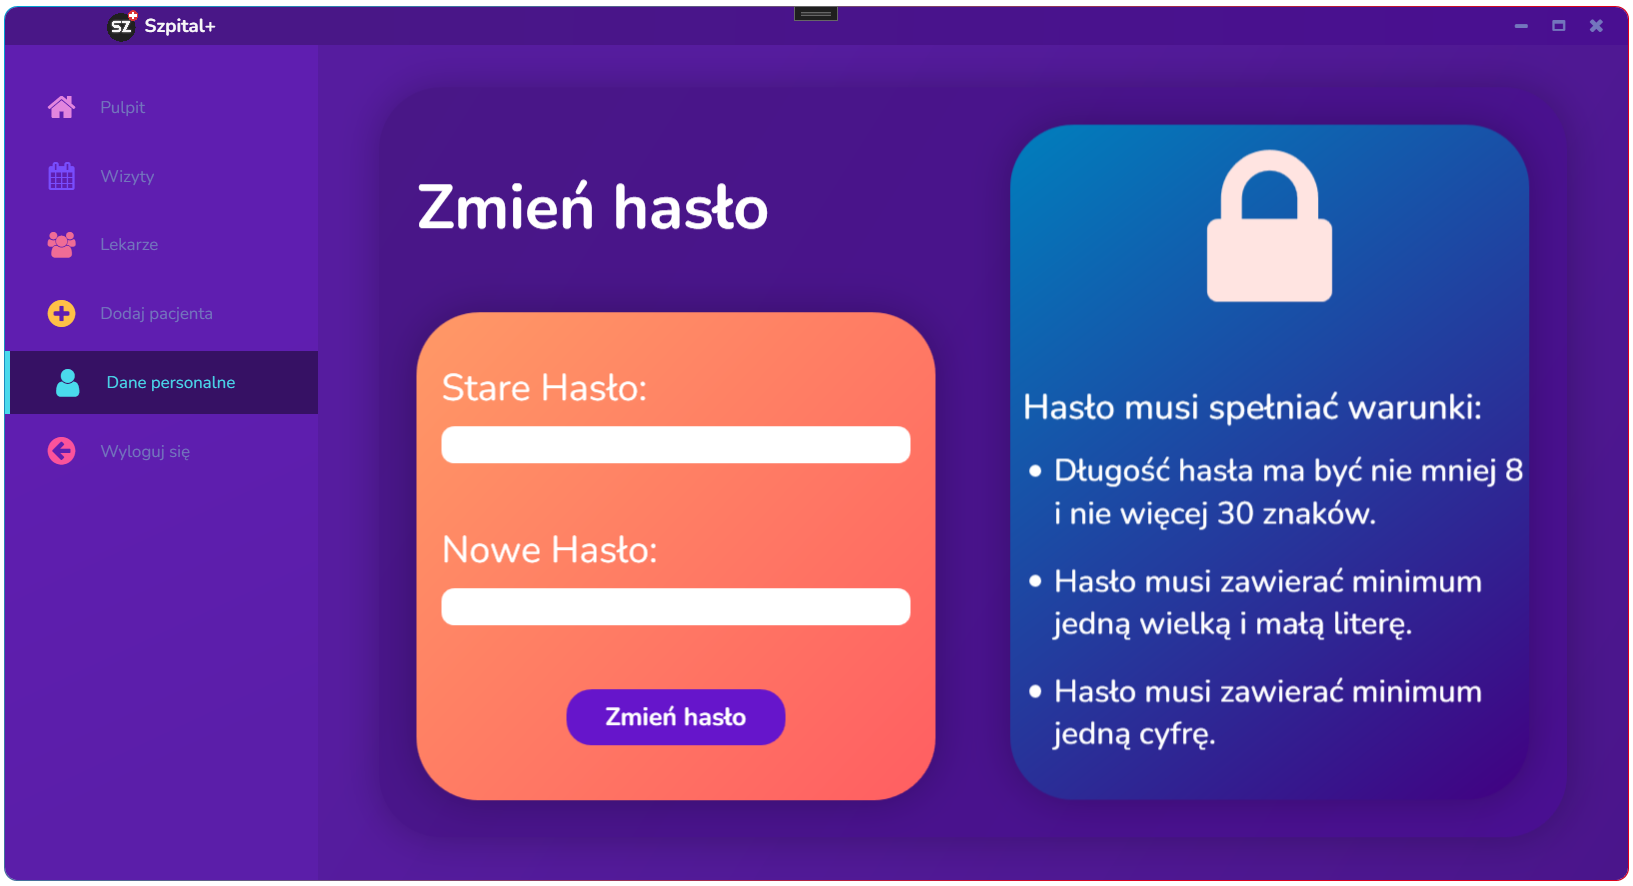
\includegraphics[height=6cm]{images/zmien_hasl.png}
    \caption{Wygląd okna \textquotedbl Zmień hasło\textquotedbl{}}
\end{center}
\end{figure}

Jeśli stare hasło nie będzie takim samym jak w bazie danych wystąpi błąd:

\begin{figure}[H]
\begin{center}
    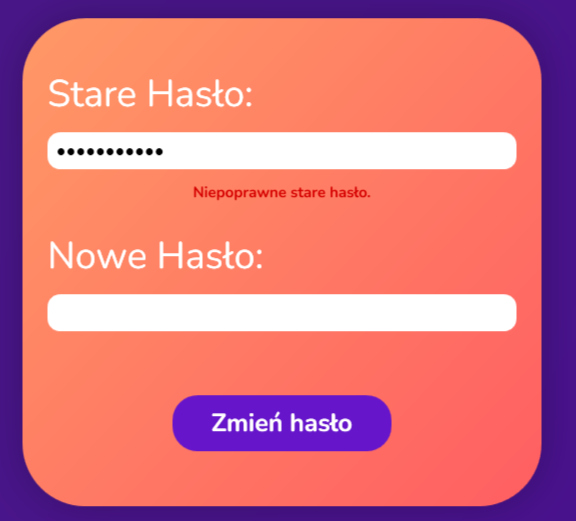
\includegraphics[height=5cm]{images/niepop_stare_hasl.png}
    \caption{Błąd przy wpisaniu starego hasła}
\end{center}
\end{figure}

\section{Sprawdzenie nowego hasła}
Sprawdzenie nowego hasła odbywa się za pomocą {\color{blue}\href{https://en.wikipedia.org/wiki/Regular_expression}{wyrażenia regularnego}}({\color{blue}\href{https://learn.microsoft.com/en-us/dotnet/standard/base-types/regular-expression-language-quick-reference}{Klasa Regex}}).

\begin{figure}[H]
\begin{center}
    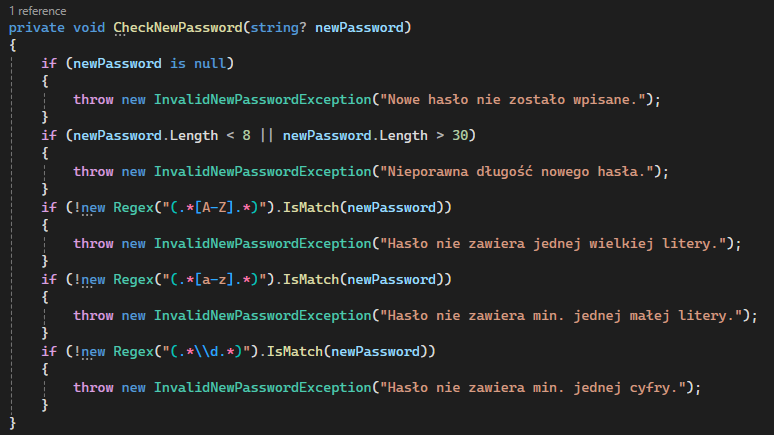
\includegraphics[height=7cm]{images/sprawdz_hasl.png}
    \caption{Metoda do sprawdzenia nowego hasła}
\end{center}
\end{figure}

\begin{figure}[H]
\begin{center}
    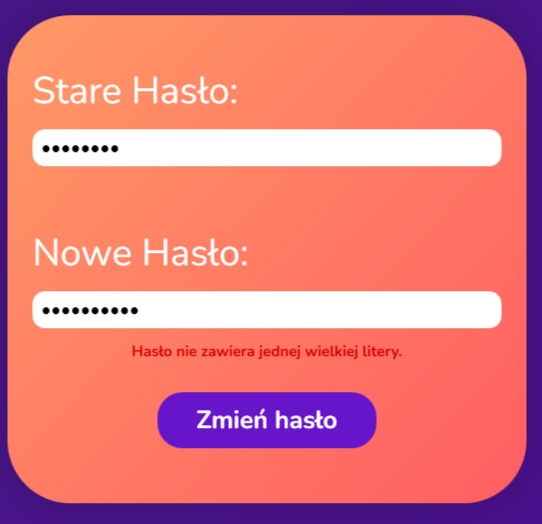
\includegraphics[height=6cm]{images/blad_nowe_hasl.png}
    \caption{Wystąpienie błędu przy nowym hasłu}
\end{center}
\end{figure}

Jeśli nowe hasło odpowiada wszystkim warunkom, pojawia się okno do zatwierdzenia operacji. Przy tym interakcja z głownem oknem jest niemożliwa dopóki użykownik anuluje lub zatwierdzi operację.

\begin{figure}[H]
\begin{center}
    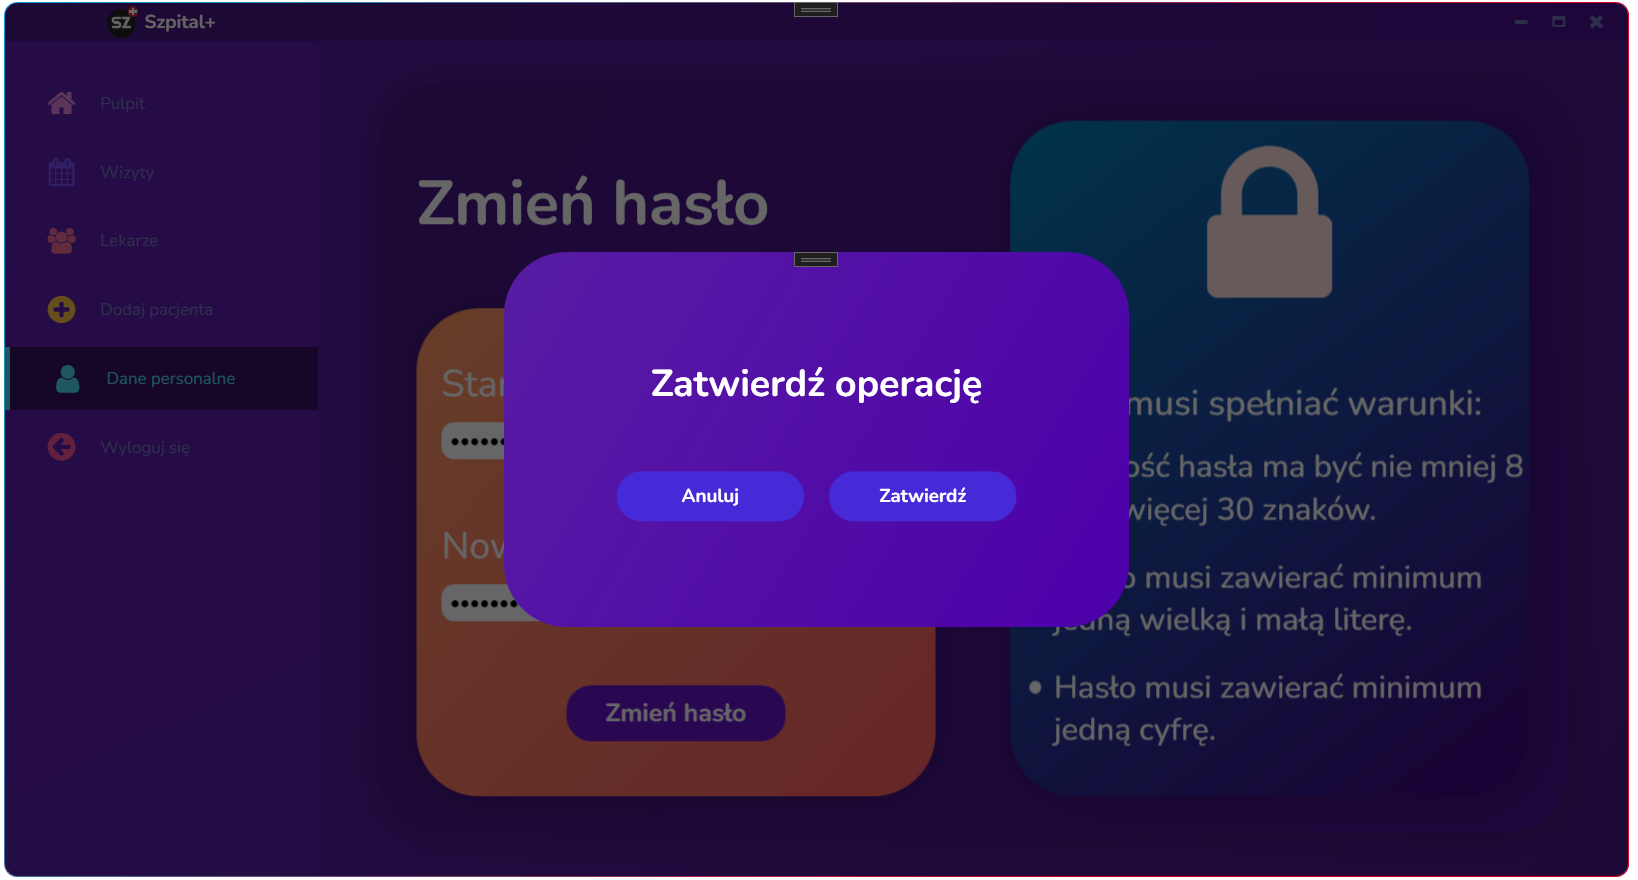
\includegraphics[height=8cm]{images/zatw_oper.png}
    \caption{Okno do zatwierdzenia operacji}
\end{center}
\end{figure}

\begin{figure}[H]
\begin{center}
    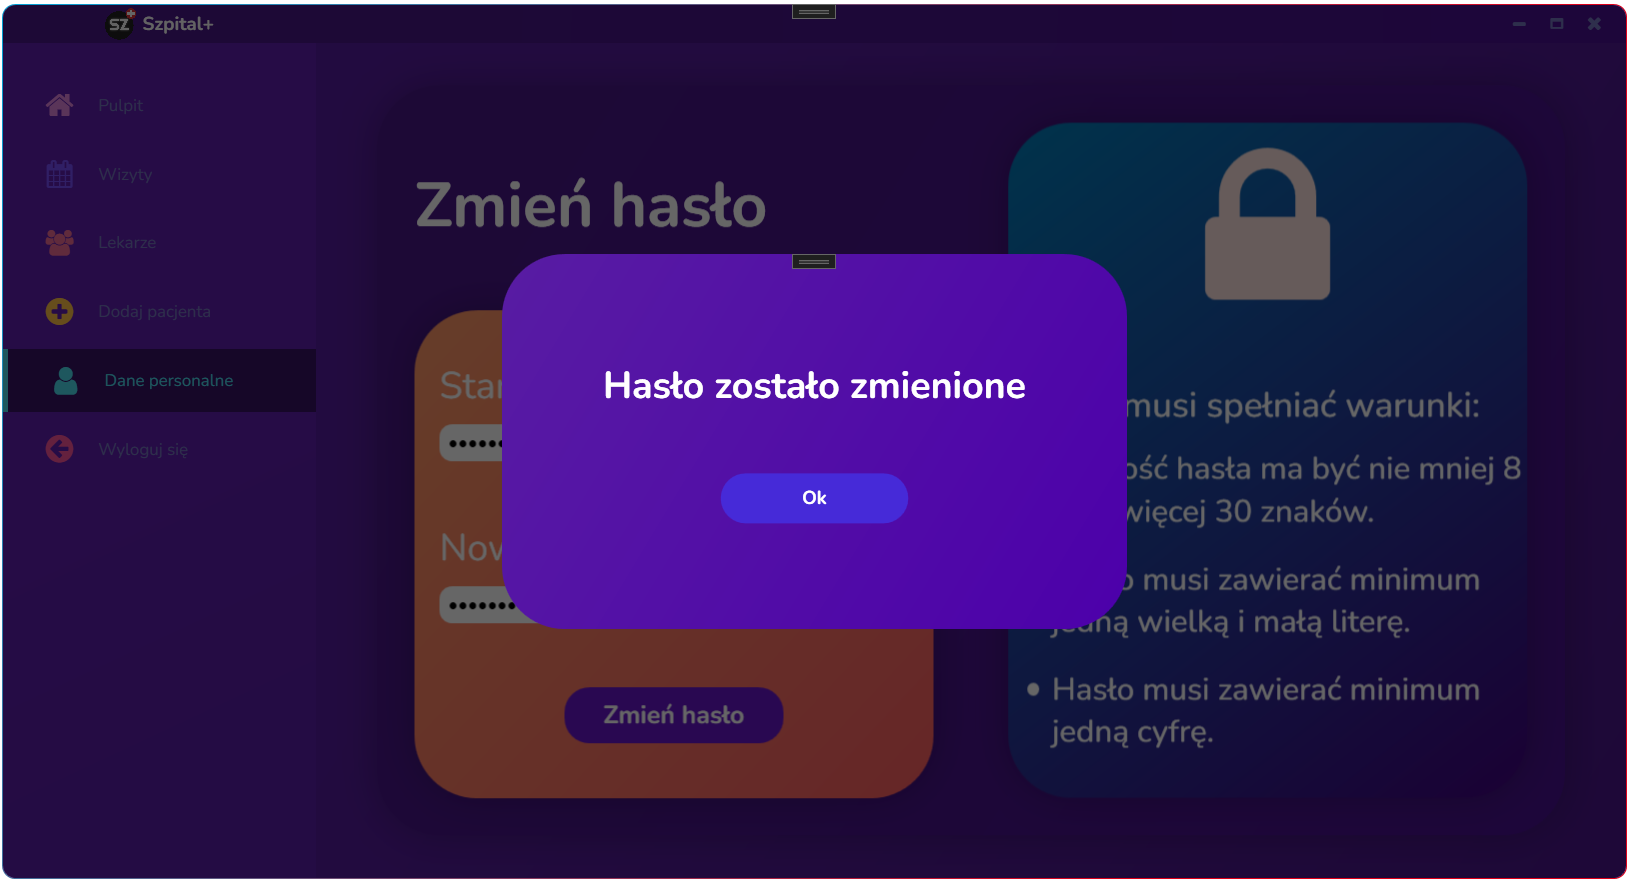
\includegraphics[height=8cm]{images/haslo_zos_zmien_katpa.png}
    \caption{Hasło zostało zmienione}
\end{center}
\end{figure}

\begin{figure}[H]
    \centering
    \subfigure{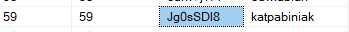
\includegraphics[width=0.4\textwidth]{images/stare_haslo_katpa.png}} 
    \subfigure{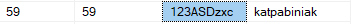
\includegraphics[width=0.4\textwidth]{images/nowe_haslo_katpa.png}}
    \caption{Stare i zmienione hasło}
\end{figure}

\newpage

\section{Okna dla recepcjonisty}
\Large\textbf{{Lekarze}}

\begin{figure}[H]
\begin{center}
    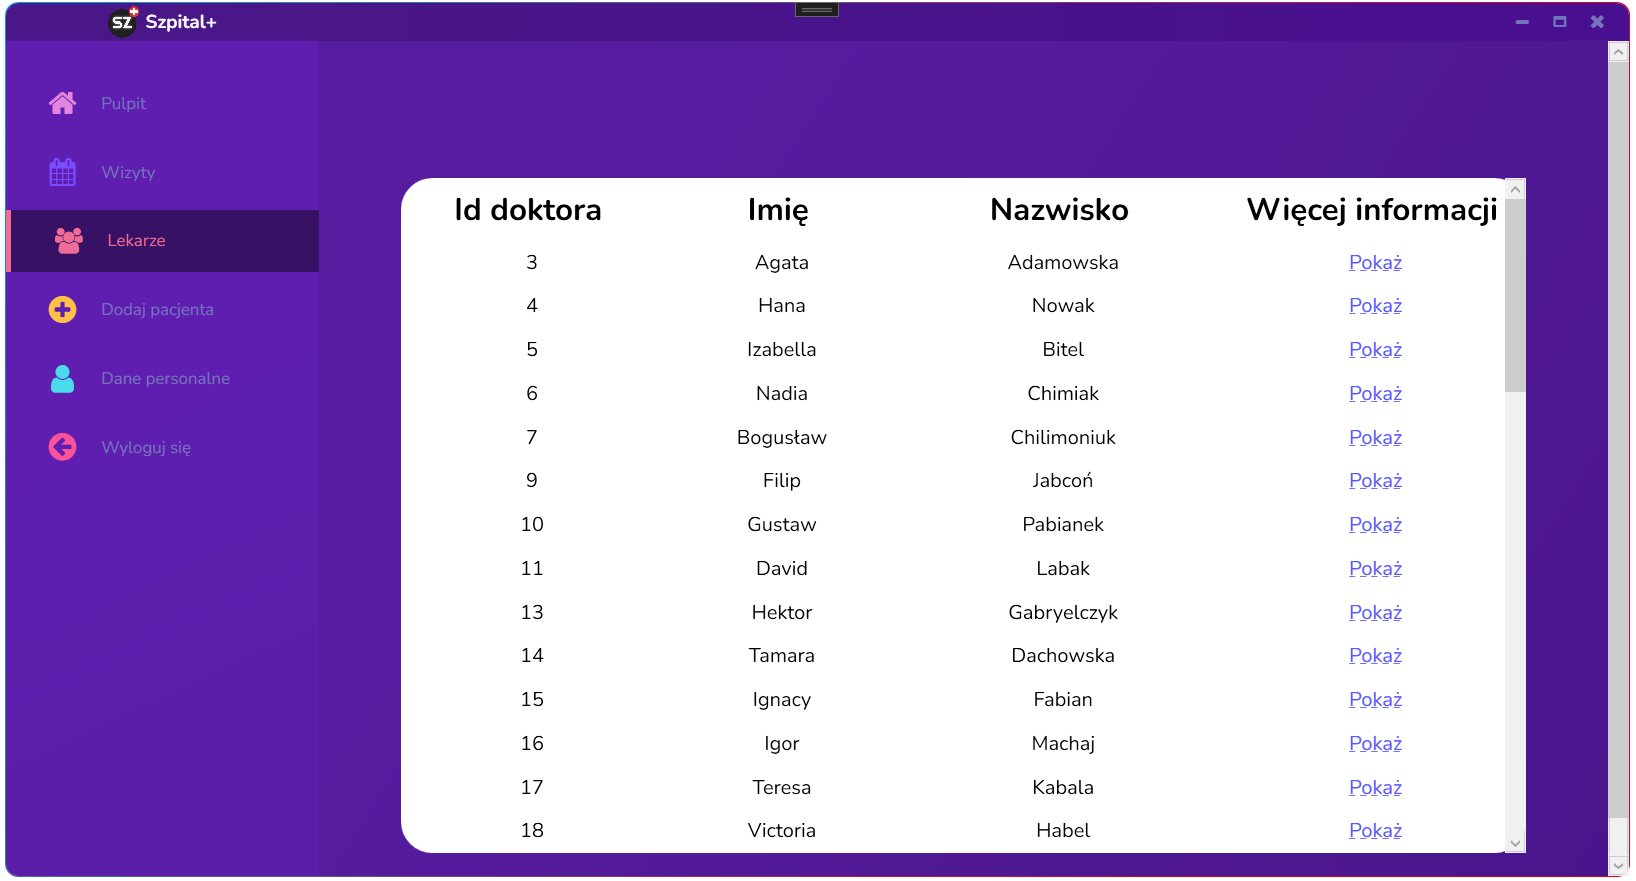
\includegraphics[height=7cm]{images/recep_lekarze.png}
    \caption{Okno recepcjonisty(Lekarze)}
\end{center}
\end{figure}

\Large\textbf{{Dodaj pacjenta}}

\begin{figure}[H]
\centering
    \subfigure{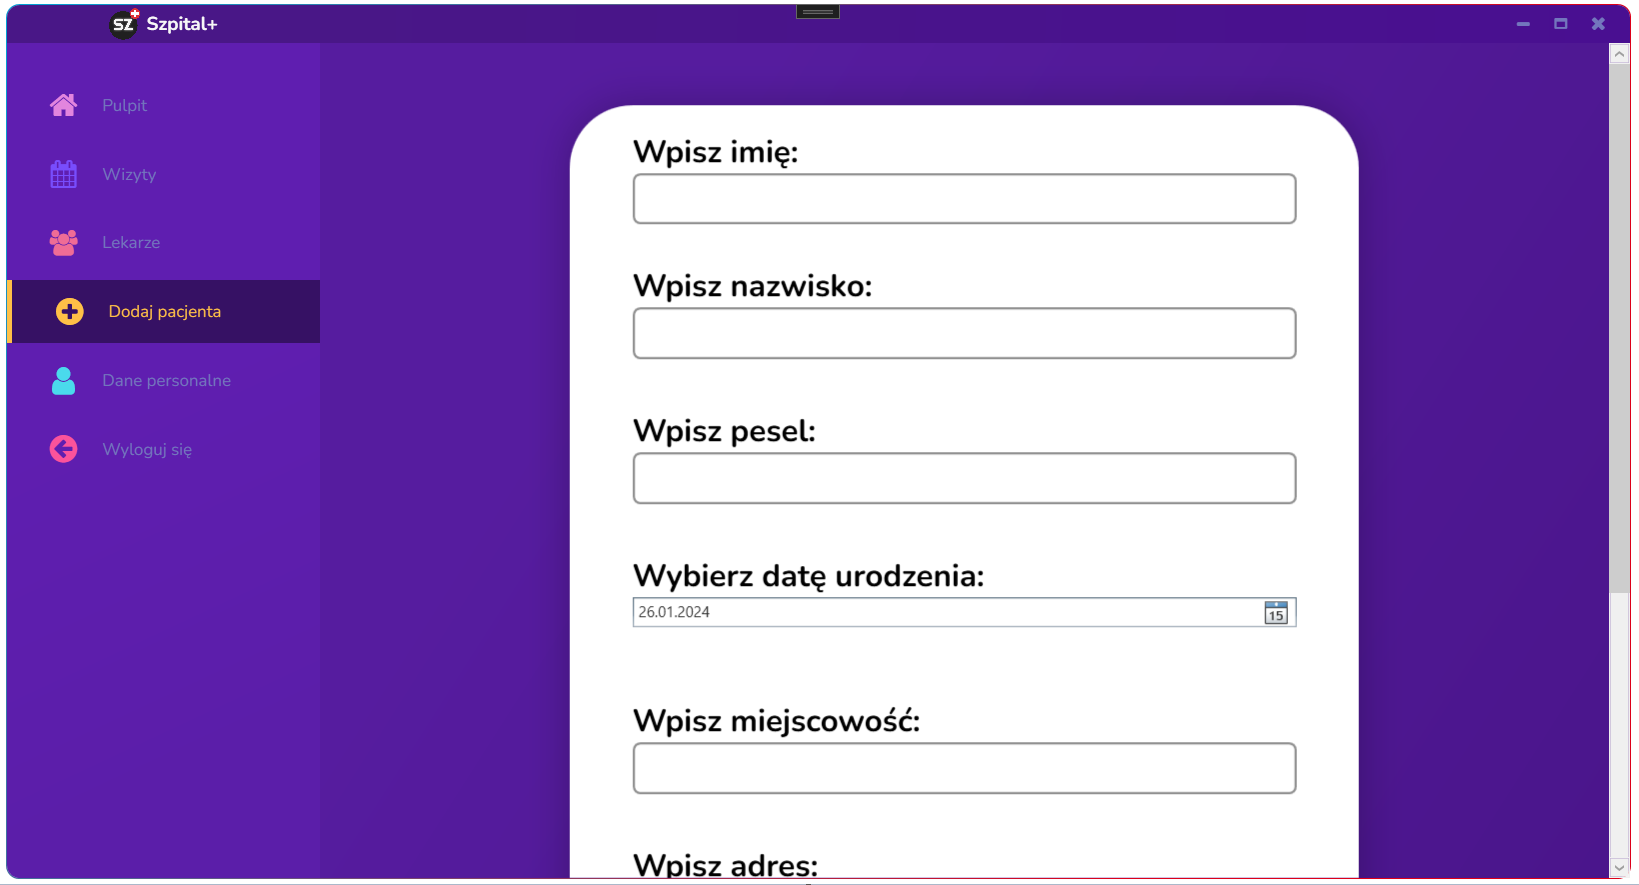
\includegraphics[width=0.6\textwidth]{images/dodaj_pacj_1.png}} 
    \subfigure{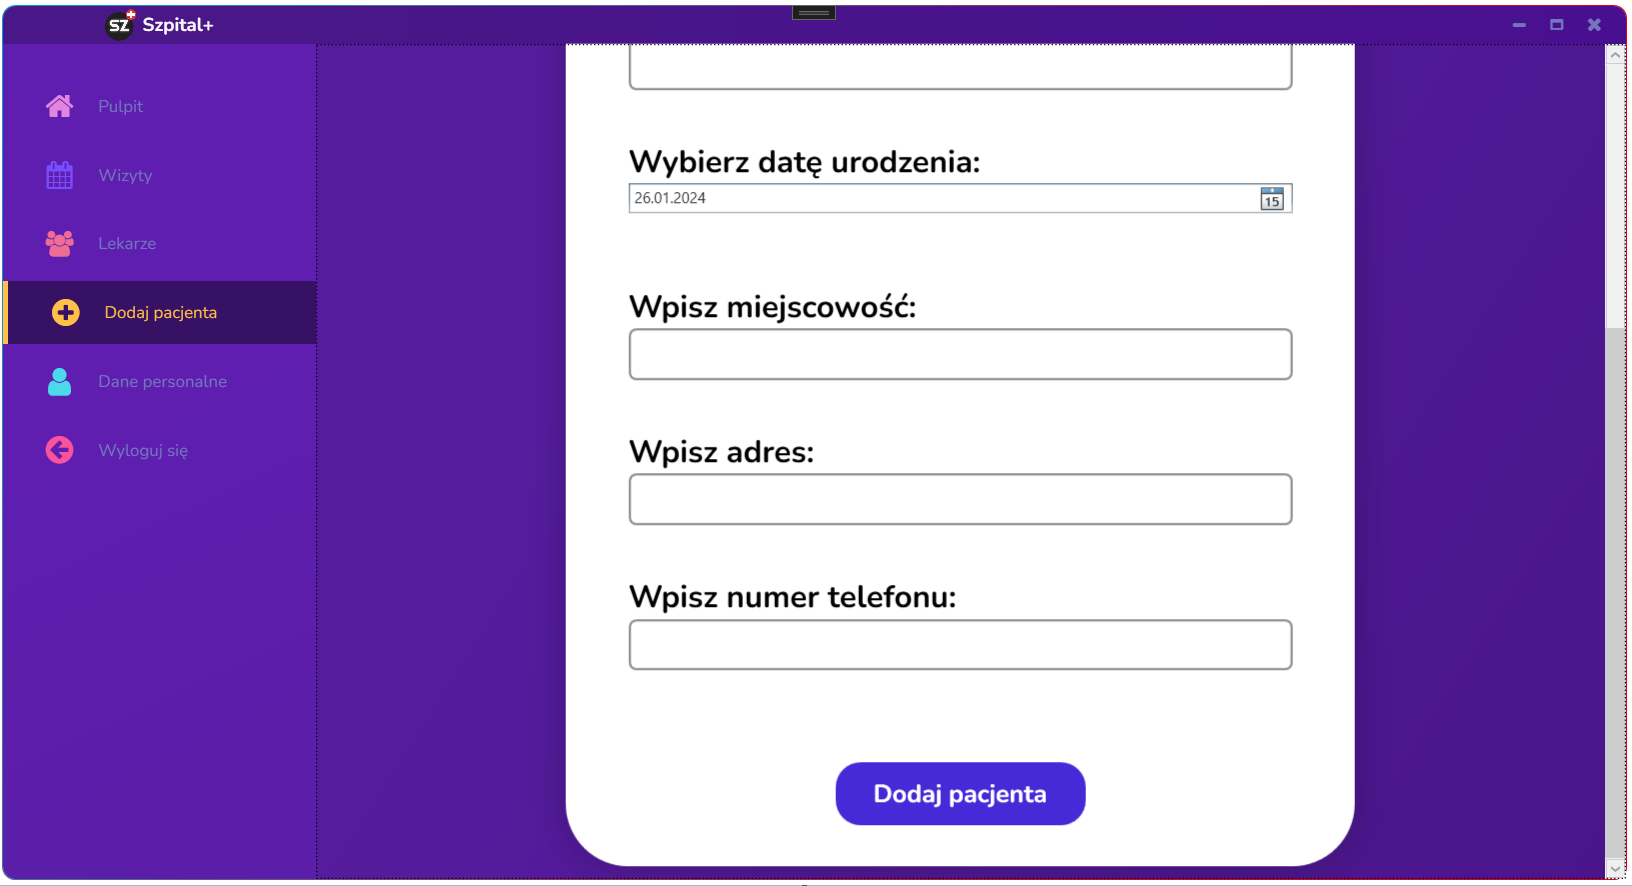
\includegraphics[width=0.6\textwidth]{images/dodaj_pacj_2.png}}
    \caption{Okno recepcjonisty(Dodaj pacjenta)}
\end{figure}

\begin{figure}[H]
    \begin{center}
    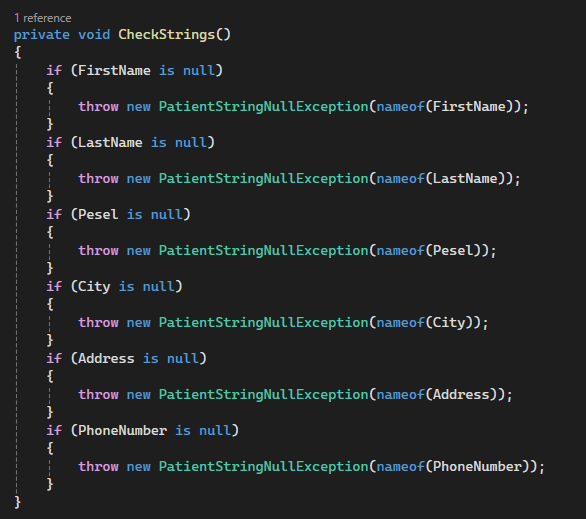
\includegraphics[height=8cm]{images/spraw_null.png}
    \caption{Sprawdzenie na puste pola}
\end{center}
\end{figure}

\begin{figure}[H]
\begin{center}
    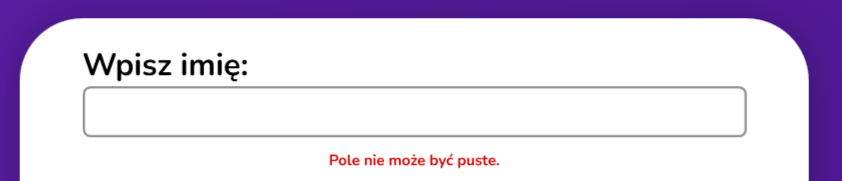
\includegraphics[height=3cm]{images/blad_wpisz_im.png}
    \caption{Wystąpienie błędu przy pustym błędzie}
\end{center}
\end{figure}

\begin{figure}[H]
\begin{center}
    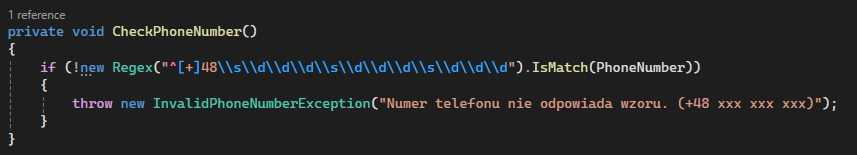
\includegraphics[height=3cm]{images/sprawd_telef.png}
    \caption{Sprawdzenie formatu telefonu}
\end{center}
\end{figure}

\begin{figure}[H]
    \begin{center}
    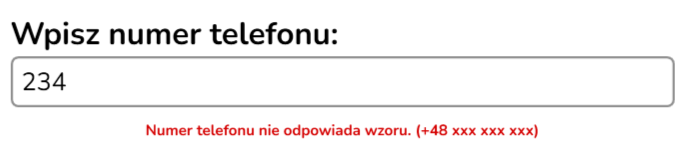
\includegraphics[height=3cm]{images/blad_telef.png}
    \caption{Błąd przy polu numeru telefonu}
\end{center}
\end{figure}

\begin{figure}[H]
\begin{center}
    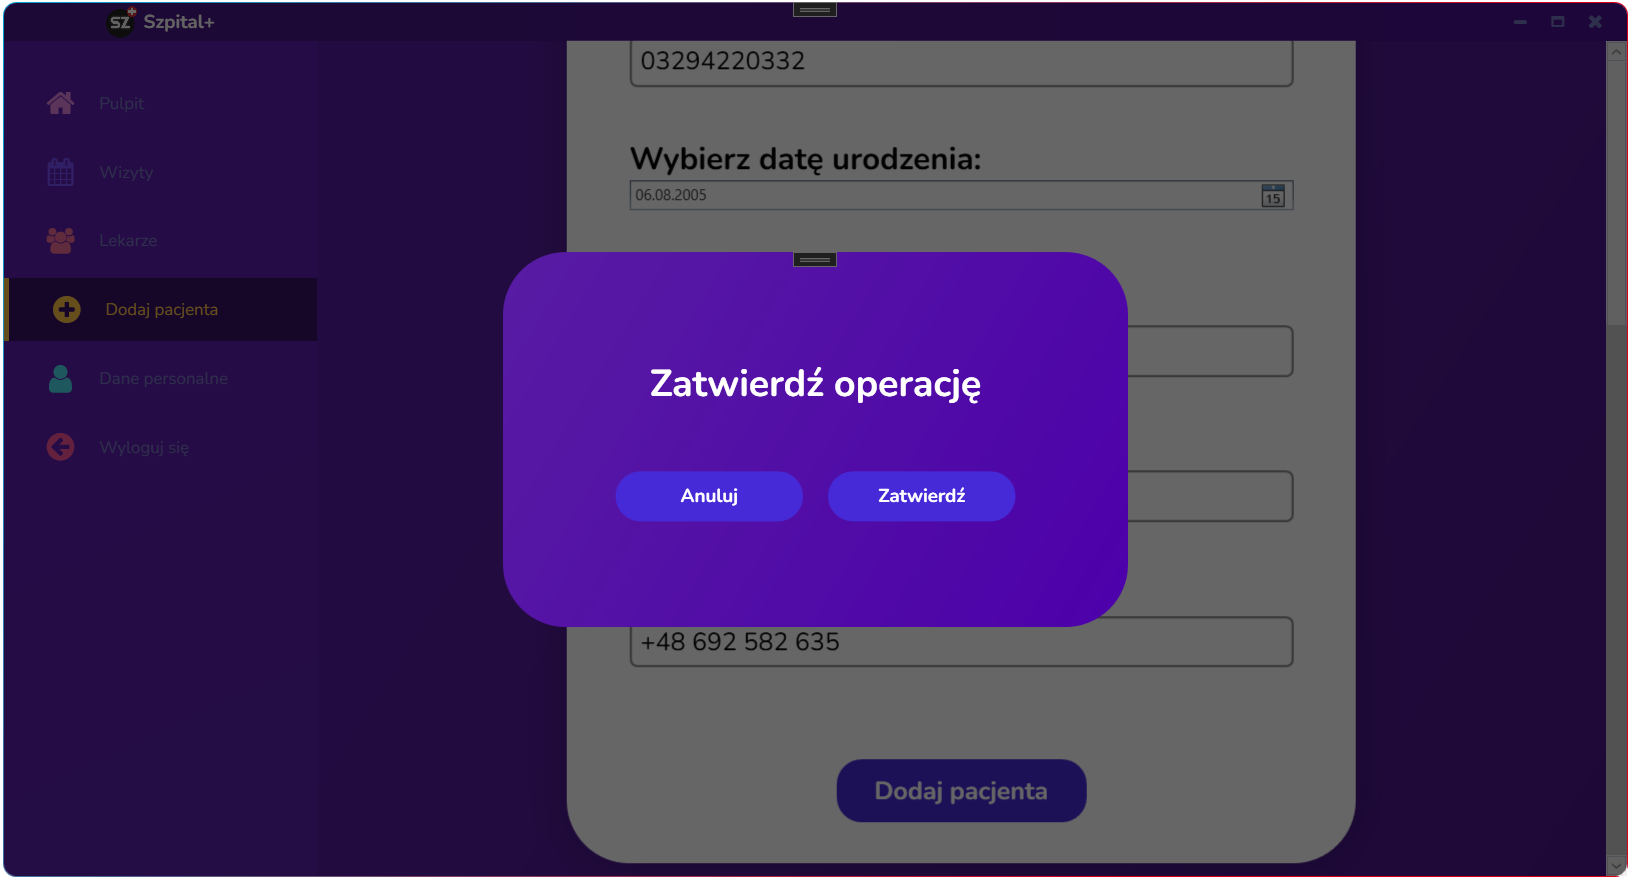
\includegraphics[height=9cm]{images/zatwr_oper_dod.png}
    \caption{Zatwierdzenie operacji}
\end{center}
\end{figure}

\begin{figure}[H]
\begin{center}
    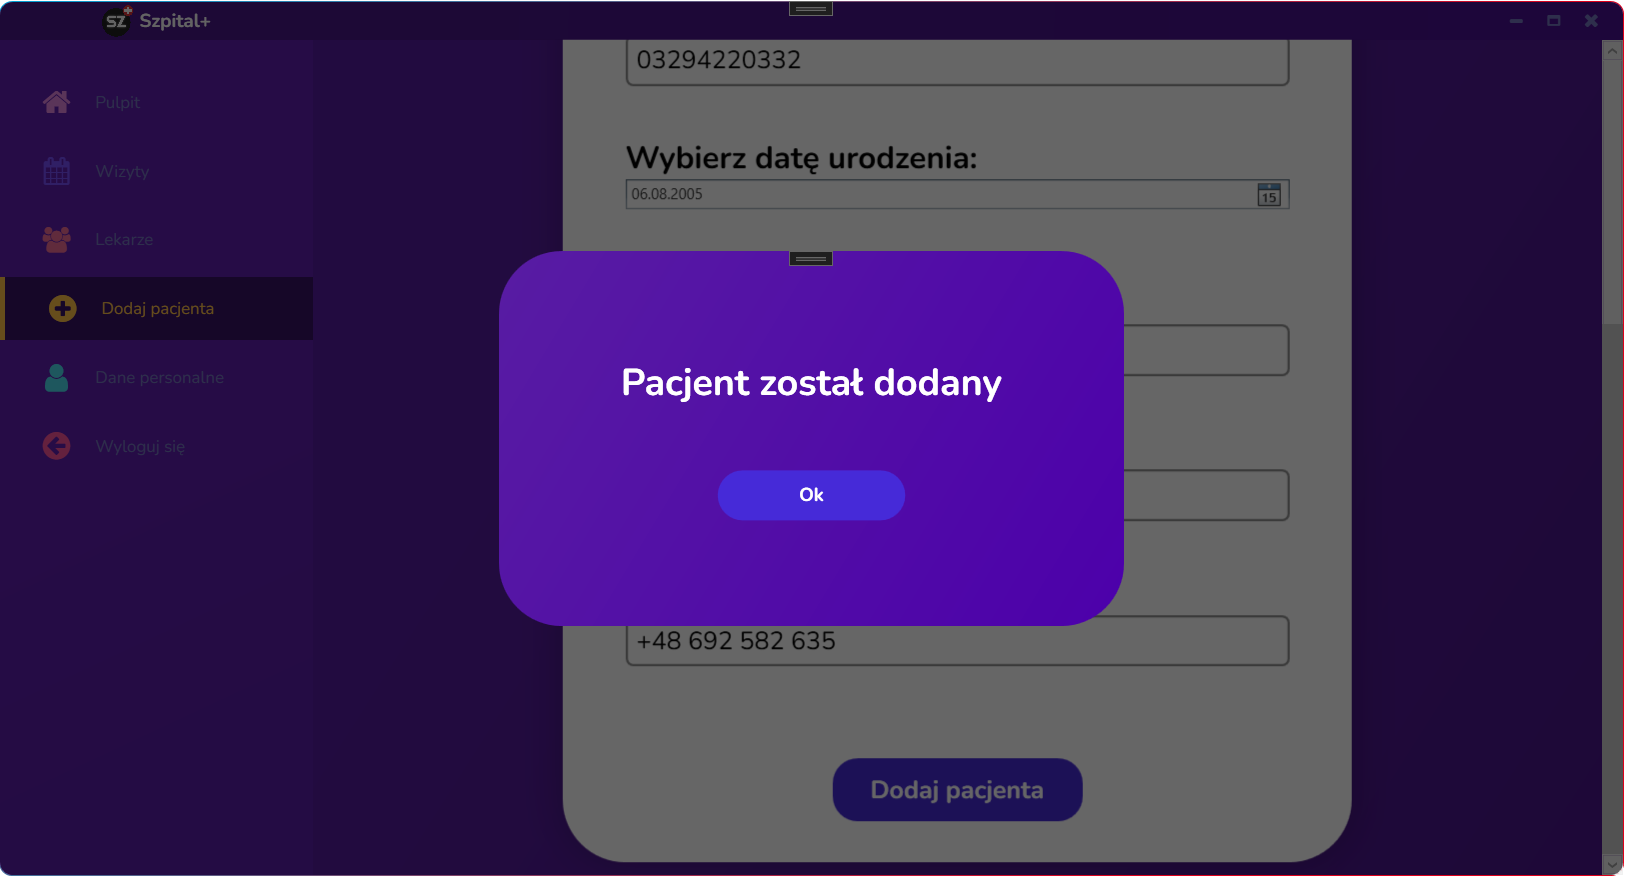
\includegraphics[height=9cm]{images/pacj_zost_dod.png}
    \caption{Pacjent został dodany}
\end{center}
\end{figure}

\begin{figure}[H]
\centering
    \subfigure{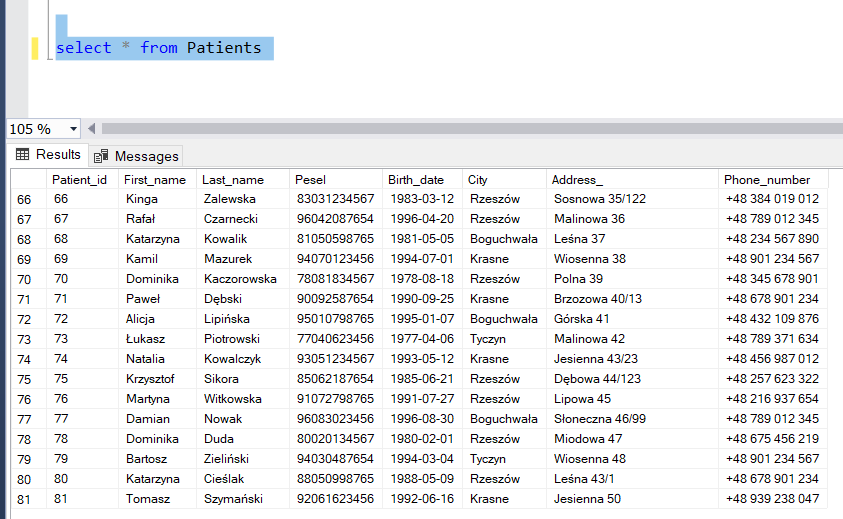
\includegraphics[width=0.6\textwidth]{images/pacjen_przed_dod.png}} 
    \subfigure{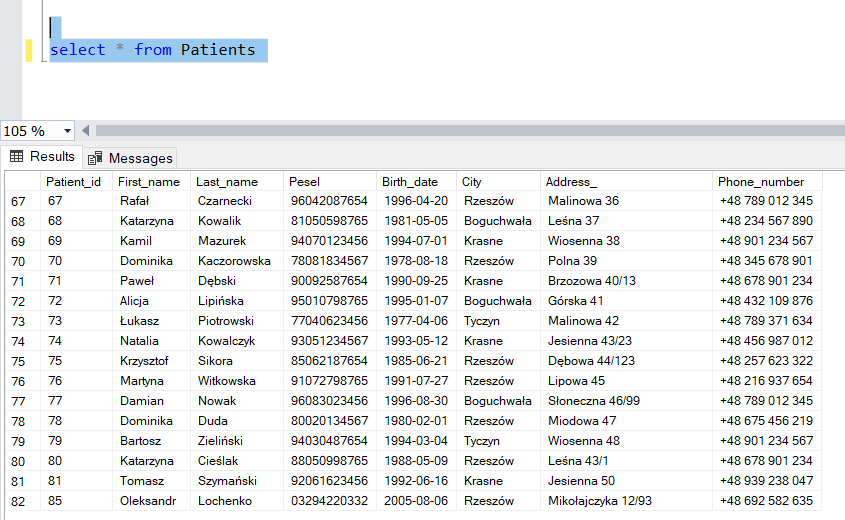
\includegraphics[width=0.6\textwidth]{images/pacjen_po_dod.png}}
    \caption{Tabela pacjentów przed i po dodaniu rekordu}
\end{figure}

\section{Okna dla głównego kierownika}
\Large\textbf{{Pracownicy}}

\begin{figure}[H]
\begin{center}
    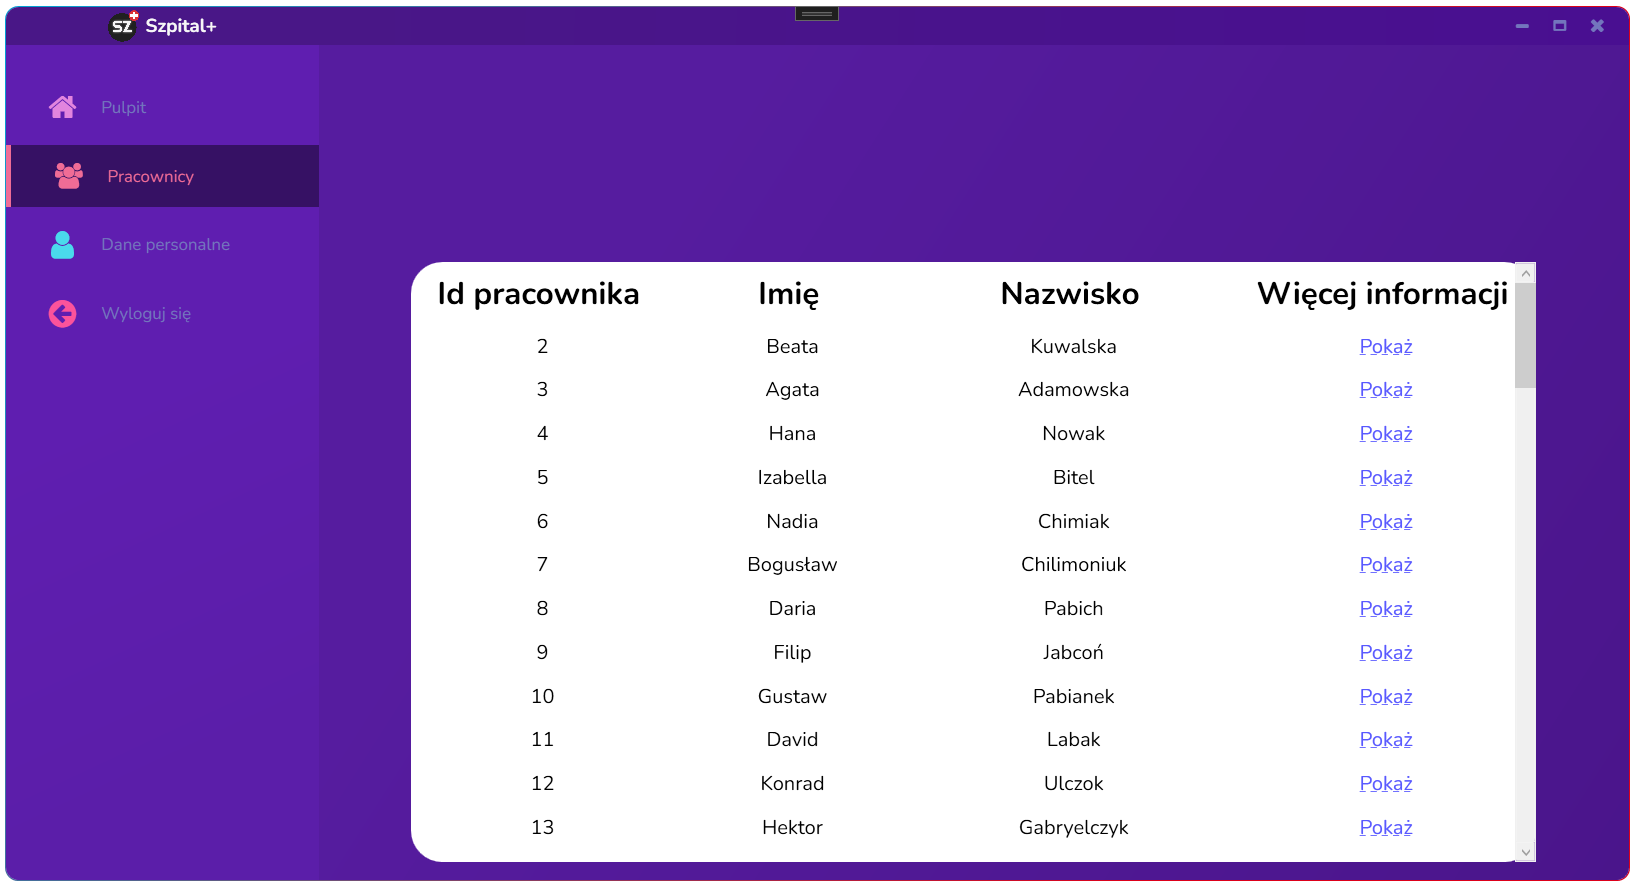
\includegraphics[height=7cm]{images/gl_kier_prac.png}
    \caption{Okno głównego kierownika(Pracownicy)}
\end{center}
\end{figure}

\section{Okna dla kierownika}
\Large\textbf{{Lekarze}}

\begin{figure}[H]
\begin{center}
    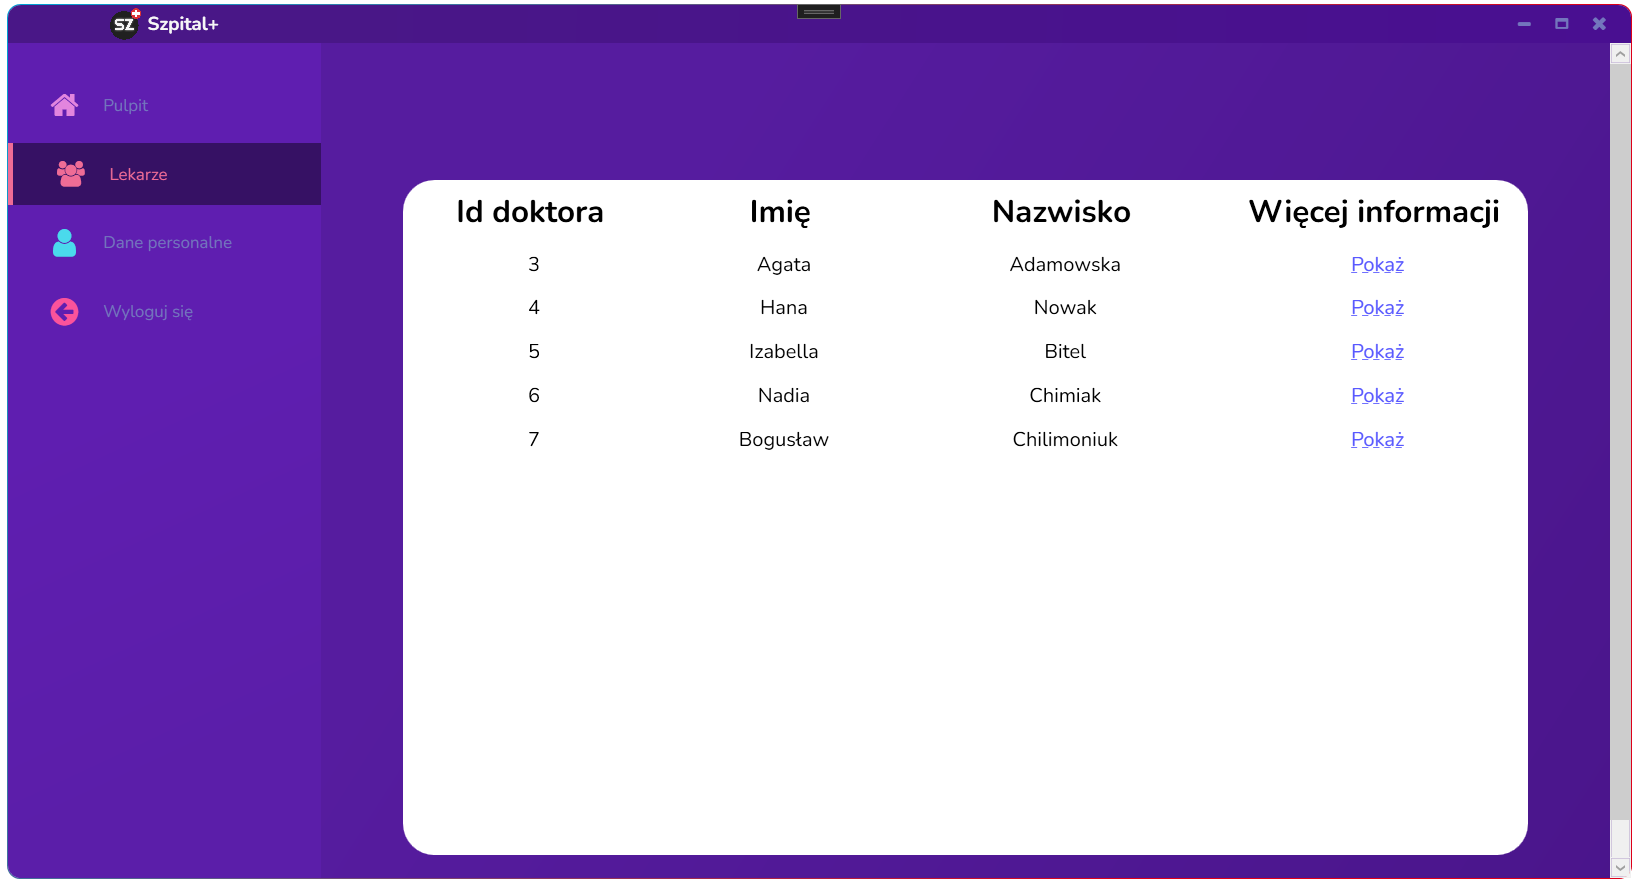
\includegraphics[height=7cm]{images/kier_lekar.png}
    \caption{Okno kierownika(Lekarze)}
\end{center}
\end{figure}

% ********** Koniec rozdziału **********
